\ProjectEntry
{mheatmap: Proportional Heatmaps with Spectral Reordering}
{Creator \& Maintainer}
{Python, NumPy, Matplotlib, Spectral Graph Theory}
{
  \bitem{Developed Python package for creating proportional heatmaps where cell sizes reflect data magnitude.}
  \bitem{Implemented spectral reordering algorithms (Fiedler vector, spectral seriation) to reveal hidden structure.}
  \bitem{Achieved 600+ GitHub stars and widespread adoption in bioinformatics, systems biology, and network analysis.}
  \bitem{Package has been cited in peer-reviewed publications and used in production data analysis pipelines.}
  \bitem{Maintained comprehensive documentation with tutorials, examples, and API reference.}
}
{assets/2002_mheatmap/02b_mheatmap.png}
{\extlink{https://github.com/qqgjyx/mheatmap}{GitHub repository} \quad \extlink{https://qqgjyx.github.io/mheatmap/}{Documentation}}
{\badge{Data Visualization} \badge{600+ Stars}}

\textbf{Technical Highlights:}
Traditional heatmaps use fixed-size cells regardless of data magnitude, making it difficult to compare values across orders of magnitude. \texttt{mheatmap} solves this by making cell areas proportional to values, creating a more intuitive visualization of hierarchical or networked data.

RMS alignment (optional) helps align permutation-invariant clusters to labels, improving interpretability and evaluation fairness (Fig.~\ref{fig:03_salinas_rms}).

\textbf{Key Features:}
\begin{itemize}[leftmargin=1.2em, itemsep=0.1em]
  \item Proportional sizing: Cell areas scale with data magnitude, preserving quantitative relationships
  \item Spectral reordering: Automatically reorders rows/columns to reveal clusters and patterns using graph Laplacian eigenvectors
  \item Flexible color mapping: Supports custom colormaps, logarithmic scaling, and diverging color schemes
  \item High-quality output: Vector graphics export (PDF, SVG) suitable for publication
  \item Easy integration: Works seamlessly with pandas DataFrames and NumPy arrays
\end{itemize}

\textbf{Use Cases:}
\begin{itemize}[leftmargin=1.2em, itemsep=0.1em]
  \item Gene expression matrices in systems biology
  \item Correlation matrices in financial data analysis
  \item Adjacency matrices for network visualization
  \item Confusion matrices in machine learning evaluation
  \item Any tabular data with hierarchical or network structure
\end{itemize}

\begin{wrapfigure}{r}{0.5\textwidth}
  \centering
  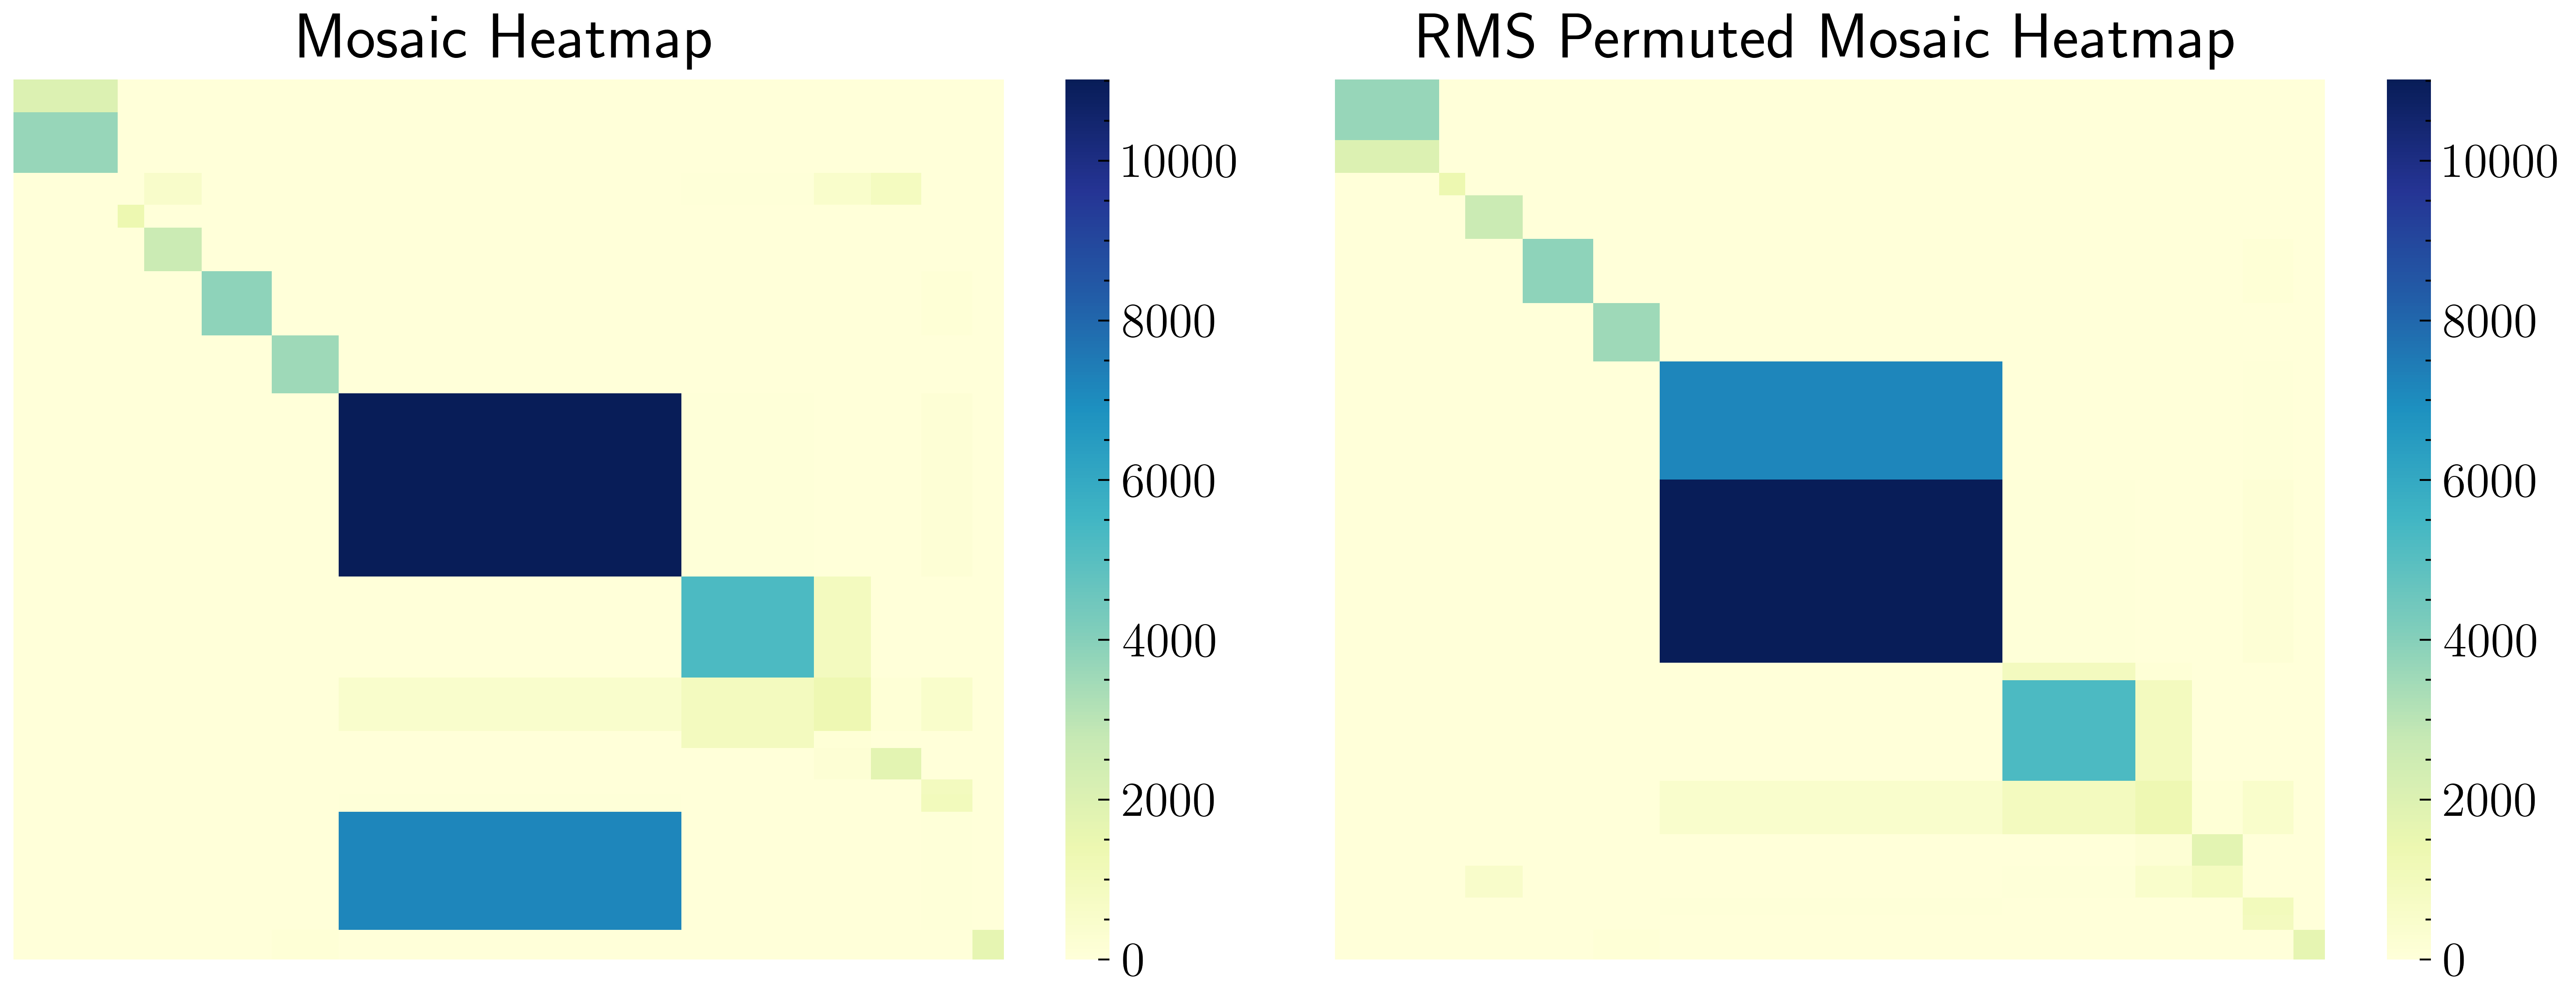
\includegraphics[width=\linewidth]{assets/2002_mheatmap/03b_salinas_rms.png}
  \caption{Salinas example: after RMS alignment, a diagonal emerges in the mosaic heatmap, improving cluster–category correspondence.}
  \label{fig:03_salinas_rms}
  \vspace{-15em}
\end{wrapfigure}

\textbf{Example Code:}
\begin{verbatim}
  import numpy as np
  import mheatmap as mh
  
  conf_mat = np.array([
      [85, 10,  5],
      [15, 70, 15],
      [ 5, 20, 75]
  ])
  
  mh.mosaic_heatmap(conf_mat)
\end{verbatim}

\textbf{Impact:}
\texttt{mheatmap} has been adopted by research groups worldwide and cited in publications spanning biology, computer science, and data science. The tool fills a gap in the Python visualization ecosystem and has become a standard tool for exploratory data analysis.
